Let $X\in\cbrak{0,1}$ represent the random variable, where $0$ represents head and 1 represents tail.  From the given information,
% given that $\to$
%\\
%No of experiment = 1000
%\\
%No of heads = 455
%\\
%No of tails = 545
%\\
%probability of comming heads = P$X=0$
%\\
\begin{align}
\pr{X=0} &= \frac{455}{1000}
\\
&= 0.45
\\
\pr{X=1} &= 1-\pr{X=0}
\\
&= 0.545
\end{align}
Codes for the above are available in
\begin{lstlisting}
solutions/1-10/codes/probexm/probexm1.py
\end{lstlisting}
%\begin{figure}[!ht]
%	\centering
%	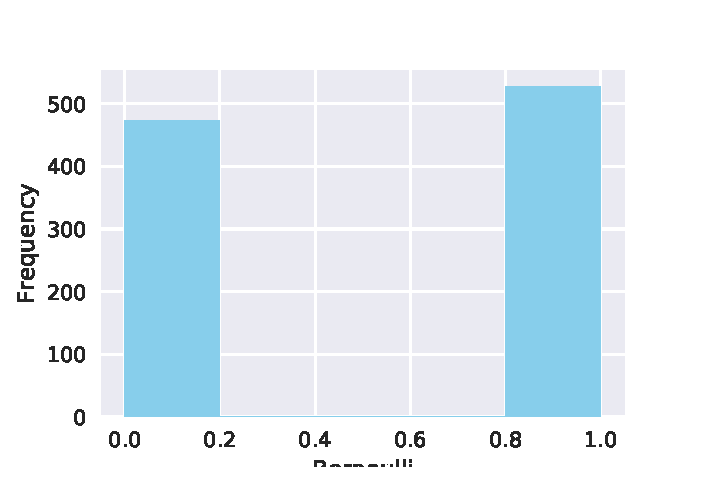
\includegraphics[width=\columnwidth]{./solutions/1-10/figures/probexm/probexm1.eps}
%	\caption{bernoulli distribution of cointo be head}
%	\label{fig:bt2}
%	\begin{lstlisting}
%	figs/probexm/probexm1.eps
%	\end{lstlisting}
%\end{figure}
